\part*{Parte B: Implementación y Análisis de Resultados}
\addcontentsline{toc}{section}{Parte B: Implementación y Análisis de Resultados}

\section{De la Teoría a la Práctica: Implementación con FEniCS}
Hemos construido el andamiaje teórico completo para resolver problemas de termoelasticidad. Ahora, es el momento de traducir este conocimiento en una herramienta de simulación funcional. En esta segunda parte, implementaremos el **Caso de Estudio: Flexión de una Tira Bimetálica** utilizando la librería FEniCS en Python.

\subsection{Caso de Estudio: Flexión de una Tira Bimetálica}
\begin{examplebox}{Caso Práctico: Termostato Bimetálico}
    \textbf{Planteamiento del Problema:} Una tira compuesta por dos metales con diferentes coeficientes de dilatación térmica (acero y cobre) está anclada en un extremo. Inicialmente a temperatura ambiente, se calienta de forma uniforme. Debido a que un material se expande más que el otro, la tira se curvará. Queremos simular este desplazamiento.
    
    \textbf{La Multifísica Clave:} El acero tiene un coeficiente de dilatación térmica ($\alpha_{\text{acero}} \approx 12 \times 10^{-6} \text{ K}^{-1}$) mucho menor que el del cobre ($\alpha_{\text{cobre}} \approx 17 \times 10^{-6} \text{ K}^{-1}$). Al calentarse, la capa de cobre intentará alargarse más que la de acero, forzando a la estructura a flexionarse.
    
    \textbf{Parámetros del Modelo:}
    \begin{itemize}
        \item \textbf{Geometría:} Dos rectángulos de $10 \text{ cm} \times 1 \text{ cm}$ unidos, formando una viga de $10 \text{ cm} \times 2 \text{ cm}$.
        \item \textbf{Propiedades Mecánicas:} Módulo de Young y Coeficiente de Poisson para el acero y el cobre.
        \item \textbf{Propiedades Térmicas:} Coeficientes de dilatación $\alpha$ para acero y cobre.
        \item \textbf{Condiciones de Contorno:}
             \begin{itemize}
                \item \textbf{Mecánicas:} Extremo izquierdo empotrado (desplazamiento cero).
                \item \textbf{Térmicas:} La temperatura inicial es de 20 $^{\circ}$C y la final es de 120 $^{\circ}$C. Resolveremos el problema estacionario final.
            \end{itemize}
    \end{itemize}
\end{examplebox}

\subsection{Implementación del Código (Versión Final)}
El siguiente script de Python resuelve el problema. La clave es separar correctamente la parte bilineal (mecánica pura) de la parte lineal (cargas térmicas) en la forma variacional.

\begin{tcolorbox}[colback=CodeBackground, title=Script de Simulación Termoelástica en FEniCS, listing only, listing options={style=pythonstyle}]
# --- 1. Importar librerías ---
from fenics import *
import matplotlib.pyplot as plt
import numpy as np
import os

# --- 2. Definir parámetros ---
L_beam = 0.1; H_metal = 0.01

E_acero = 200e9; nu_acero = 0.3; alpha_acero = 12e-6
lambda_acero = E_acero*nu_acero/((1+nu_acero)*(1-2*nu_acero))
mu_acero = E_acero/(2*(1+nu_acero))

E_cobre = 120e9; nu_cobre = 0.34; alpha_cobre = 17e-6
lambda_cobre = E_cobre*nu_cobre/((1+nu_cobre)*(1-2*nu_cobre))
mu_cobre = E_cobre/(2*(1+nu_cobre))

T_inicial = 20.0; T_final = 120.0

# --- 3. Malla y Subdominios ---
mesh = RectangleMesh(Point(0,-H_metal), Point(L_beam, H_metal), 40, 20)
subdomains = MeshFunction("size_t", mesh, mesh.topology().dim())
class Acero(SubDomain):
    def inside(self, x, on_boundary): return x[1] <= 0.0 + DOLFIN_EPS
class Cobre(SubDomain):
    def inside(self, x, on_boundary): return x[1] >= 0.0 - DOLFIN_EPS
subdomain_acero=Acero(); subdomain_cobre=Cobre()
subdomain_acero.mark(subdomains, 0); subdomain_cobre.mark(subdomains, 1)
dx = Measure('dx', domain=mesh, subdomain_data=subdomains)

# --- 4. Espacio de Funciones y BC ---
V_u = VectorFunctionSpace(mesh, 'P', 2)
def empotramiento_borde(x, on_boundary): return on_boundary and near(x[0], 0)
bc_mecanico = DirichletBC(V_u, Constant((0, 0)), empotramiento_borde)

# --- 5. Forma Débil ---
u = TrialFunction(V_u); v = TestFunction(V_u)
T = Constant(T_final)
def epsilon(u): return 0.5*(grad(u) + grad(u).T)

lmbda=Expression('x[1]>=0?l_cobre:l_acero',l_cobre=lambda_cobre, l_acero=lambda_acero, degree=0)
mu=Expression('x[1]>=0?mu_cobre:mu_acero', mu_cobre=mu_cobre, mu_acero=mu_acero, degree=0)
alpha=Expression('x[1]>=0?a_cobre:a_acero', a_cobre=alpha_cobre, a_acero=alpha_acero, degree=0)

def sigma_mec(u): return lmbda*tr(epsilon(u))*Identity(len(u)) + 2*mu*epsilon(u)
def sigma_th(T): return -(3*lmbda+2*mu)*alpha*(T-T_inicial)*Identity(len(u))

a_form = inner(sigma_mec(u), epsilon(v)) * dx
L_form = -inner(sigma_th(T), epsilon(v)) * dx

# --- 6. Resolver y Guardar ---
u_sol = Function(V_u, name="Desplazamiento")
solve(a_form == L_form, u_sol, bc_mecanico)
if not os.path.exists("termoelasticidad"): os.makedirs("termoelasticidad")
vtkfile = File('termoelasticidad/desplazamiento.pvd'); vtkfile << u_sol

# --- 7. Post-procesamiento ---
x_coords=np.linspace(0, L_beam, 101); deflexiones=[]
for x in x_coords:
    try: deflexiones.append(u_sol(x, H_metal)[1])
    except: deflexiones.append(np.nan) # Añadir NaN si el punto está fuera
plt.figure(figsize=(10,6)); plt.plot(x_coords, deflexiones, color='#001F3F', lw=2.5)
plt.title('Deflexión del Borde Superior de la Tira Bimetálica'); plt.xlabel('Posición (m)'); plt.ylabel('Deflexión Vertical (m)'); plt.grid(True,ls='--');
plt.savefig('deflexion_bimetalica.png')
\end{lstlisting}
\end{tcolorbox}

\subsection{Análisis de Resultados y Visualización}
La ejecución del script genera los datos para visualizar y cuantificar el fenómeno.
\begin{figure}[h!]
\centering
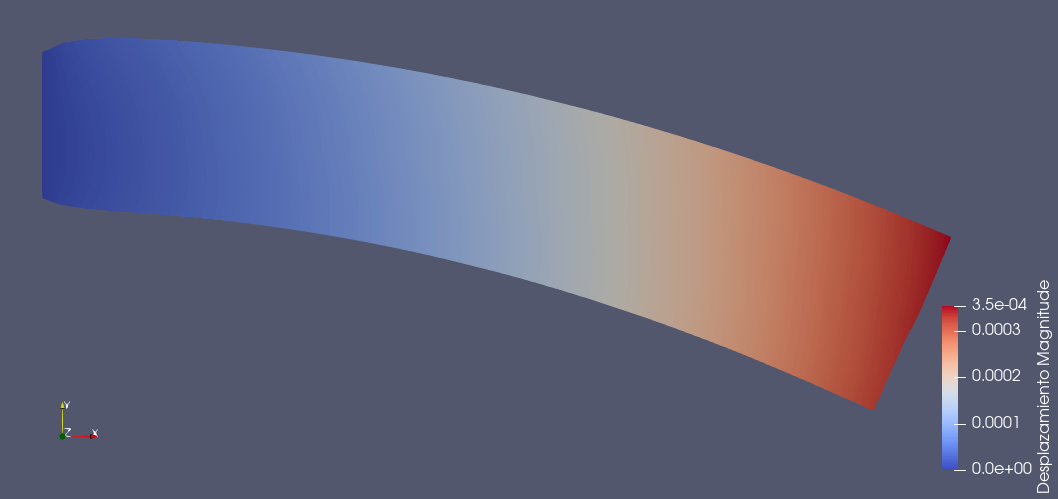
\includegraphics[width=0.9\textwidth]{paraview_deformacion.png} % <-- Reemplaza con tu imagen de ParaView
\caption{Visualización del campo de desplazamientos (magnificado) en ParaView. La tira se curva hacia abajo, confirmando que la capa superior (cobre, con mayor $\alpha$) se expande más que la inferior (acero), induciendo un momento flector interno.}
\end{figure}
\begin{figure}[h!]
\centering
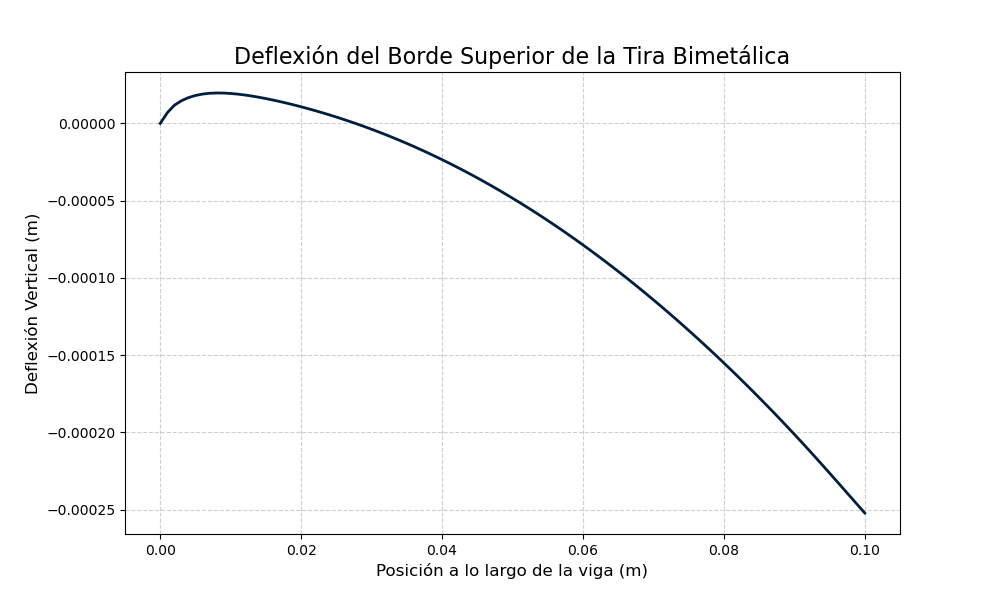
\includegraphics[width=0.8\textwidth]{deflexion_bimetalica.png} % <-- Esta imagen la genera el script
\caption{Gráfico de la deflexión vertical ($u_y$) del borde superior de la viga ($y=H_
\text{metal}$). La curva cuantifica el efecto del actuador, mostrando una deflexión máxima en el extremo libre.}
\end{figure}

\section{Conclusión General del Módulo}
En este módulo, hemos cruzado la frontera hacia la simulación multifísica, uniendo la mecánica de sólidos con la transferencia de calor. Al implementar y analizar un problema de ingeniería clásico como la tira bimetálica, hemos completado el ciclo desde la teoría física hasta el análisis de resultados cuantitativos, estableciendo un flujo de trabajo que genera conocimiento para la toma de decisiones de diseño informadas.
